\vspace{-1em}
\section{Method}
\label{sec:method}
\vspace{-0.5em}



\subsection{Problem Setting}
\vspace{-0.5em}
Given an RGB image $\mathbf{I}$ and a user-provided prompt $p$ (mask, box, or point), our goal is to identify the same object throughout a video sequence with consistent segmentation, avoiding false correspondences or identity switches across frames.
Previous approaches often fail at this goal.
\textbf{2D-based methods} (e.g., SAM2~\cite{ravi2024sam2}) rely solely on appearance features, making them sensitive to viewpoint or distance changes and prone to confusion among visually similar objects~\cite{videnovic2025distractor}, leading to frequent tracking failures over longer sequences.
\textbf{3D-based methods} (e.g., Mask3D~\cite{schult2022mask3d}, OpenYOLO3D~\cite{boudjoghra2024open}, EmbodiedSAM~\cite{xu2024esam}) localize objects using 3D mask proposals or dense 2D masks with camera poses, but require SfM or similar pipelines whose runtime and complexity grow rapidly with the number of frames, making them impractical for long sequences.
One might instead apply a 3D segmentation model on predicted geometry (e.g., point clouds from MUSt3R). However, geometry quality, especially in dynamic scenes, limits downstream segmentation reliability. Moreover, current 3D segmentation models are mainly offline, unsuitable for real-time scenarios such as robotic navigation. More importantly, large-scale training data is far more abundant in the 2D video domain, and the SAM2 model we adopt provides a strong, promptable 2D prior difficult to match with current 3D alternatives. Our method leverages this advantage by using 3D information only as a lightweight association cue rather than a hard prerequisite, maintaining a 2D segmentation framework. Specifically, we encourage geometry-consistent feature matching, enabling the model to identify the same object by recognizing its correspondence in 3D space.
% Given an RGB image $\mathbf{I}$ and a user-provided prompt $p$ (which can be a mask, box, or point), our goal is to identify the same object throughout a video sequence while maintaining consistent segmentation, i.e., avoiding false correspondences or identity switches across frames.
% Previous approaches often fail to achieve this goal. 
% \textbf{2D-based methods} (e.g., SAM2~\cite{ravi2024sam2}) rely solely on image-space appearance features, and thus are sensitive to camera viewpoint or distance changes. 
% They also struggle with visually similar or confusing objects, as partially addressed by DAM4SAM~\cite{videnovic2025distractor}, leading to frequent tracking failures as the frame sequence grows longer. 
% \textbf{3D-based methods} (e.g., Mask3D~\cite{schult2022mask3d}, OpenYOLO3D~\cite{boudjoghra2024open}, EmbodiedSAM~\cite{xu2024esam}) attempt to localize objects in space using 3D mask proposals or dense 2D masks combined with camera poses, but this requires running structure-from-motion (SfM) or similar pipelines. 
% As the number of video frames increases, both runtime and computational complexity grow rapidly, making these approaches impractical for long sequences or large scenes.
% To address these limitations, one might consider applying a 3D segmentation model on predicted geometry (e.g., point clouds from MUSt3R); however, the quality of such geometry, especially in challenging cases like dynamic scenes, significantly limits the reliability of downstream 3D segmentation. Besides, current 3D segmentation models are mainly offline, which might not be suitable for a real-time scenario, e.g., robotic navigation. More importantly, large-scale training data is far more abundant in the 2D video domain than in 3D, and the SAM2 model we adopt provides a strong, promptable 2D prior that is difficult to match with current 3D segmentation models. Our method leverages this advantage while using 3D information only as a lightweight association cue, rather than as a hard prerequisite, while maintaining a 2D segmentation framework.
% Specifically, we encourage the model to perform feature matching that is geometry-consistent, enabling it to identify the same object by recognizing its correspondence in 3D space.


\vspace{-0.5em}
\subsection{Architecture}
\vspace{-0.5em}
The overall pipeline is shown in \cref{fig:pipline}.
For each video frame $i$, our model extracts two complementary feature streams that capture appearance cues and multi-view geometric consistency. 
First, the frame is processed by the SAM2 vision encoder, producing a 2D appearance feature map $F_{\mathrm{2D}}^{i}$. 
In parallel, the same frame is passed into MUSt3R, which attends to its own multi-view memory through MUSt3R's internal cross-attention mechanism, yielding a geometry-aware feature map $F_{{3D}}^{i}$. Next, $F_{{2D}}^{i}$ and $F_{{3D}}^{i}$ are fused into a refined representation $F_{{merged}}^{i}$. The merged feature is processed by the memory attention module and the mask decoder, and is finally encoded by the memory encoder to produce memory features that will be referenced by future frames. We provide comparisons of different memory selection methods in \cref{tab:memory-selection}.


\vspace{-1em}
\subsubsection{Feature Merging.}

\begin{figure*}[t]
  \centering
\vspace{-3mm}
  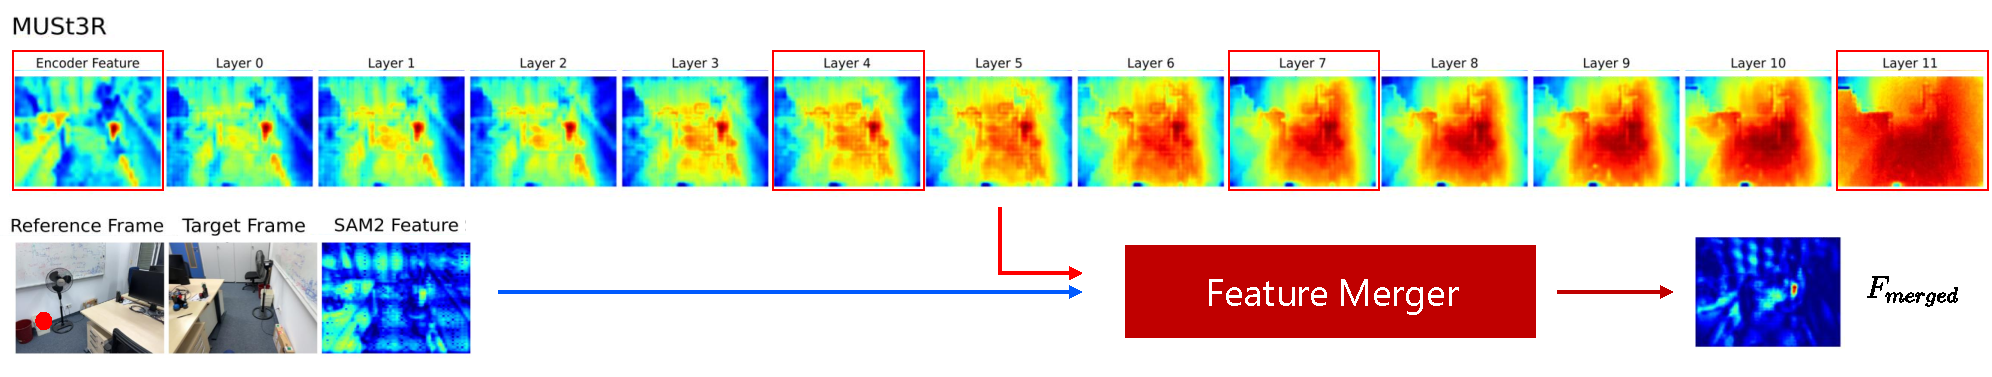
\includegraphics[width=\linewidth]{figs/FeatureMerging.pdf}
  \vspace{-6mm}
  \caption{\textbf{Illustration of Features for Feature Merging.} The heat map is computed using the cosine similarity between the red query point and the target frame. As illustrated in the lower row, vanilla SAM2 fails under large viewpoint changes. In contrast, as the MUSt3R feature hierarchy gradually shifts from semantic correspondence toward the point-cloud domain, we select intermediate layers to preserve both semantic relevance and geometric structure. By combining MUSt3R's geometric cues with SAM2's visual semantics, the merged feature $F_{{merged}}$ provides a significantly more reliable localization of the target object.
  }
  \label{fig:feature-merging}
\vspace{-3mm}
\end{figure*}

As shown in \cref{fig:feature-merging}, SAM2 becomes unreliable when the object reappears or when the viewpoint changes drastically. The heat map in the lower row demonstrates that SAM2 cannot reliably associate the query point with its target under large angular differences, revealing its limited capacity to maintain object identity when the visual appearance changes substantially.

To address this issue, we enhance SAM2 with MUSt3R features $F_{{3D}}^{i}$. The upper row of \cref{fig:feature-merging} visualizes MUSt3R activations across depth. Early layers preserve a clearer correspondence pattern with the query point, while deeper layers produce more diffuse responses. This shift reflects MUSt3R’s progression toward point-cloud decoding: the representation becomes more geometry-oriented but less semantically aligned with the 2D query. Consequently, relying solely on either early or late layers is insufficient; early layers lack explicit geometric structure, whereas late layers lose semantic clarity. We therefore sample MUSt3R features from both early and late stages to capture complementary information.

These multi-level MUSt3R features are processed by our \textbf{Feature Merger}, which jointly performs cross-attention fusion and convolutional refinement. The cross-attention blocks first integrate the sampled MUSt3R layers into a single geometry-aware feature, aligning information from different depths. 
Specifically, as shown in \cref{fig:feature-merging}, we take the MUSt3R encoder feature at the shallowest sampled depth, i.e., the most semantically rich layer, as the initial input to the Feature Merger. It first passes through a self-attention block to establish an initial semantic representation. The remaining sampled MUSt3R features are then incorporated one by one through a sequence of cross-attention layers, where the current merged representation acts as the query, and each additional MUSt3R feature provides the key–value pairs. In this way, the Feature Merger progressively integrates information from both shallow and deeper stages of MUSt3R.
The output is then fed into a convolutional stage that merges it with SAM2’s 2D feature $F_{2D}$ for restoring fine spatial detail. We further compare different 3D foundation models in \cref{tab:3D_backbone}, and more architectural details and comparisons are provided in the supplementary materials.

The final merged feature, $F_{{merged}}$, retains SAM2’s high-resolution, segmentation-aware appearance cues while incorporating MUSt3R’s geometry-aware consistency, enabling robust object localization even under severe viewpoint changes. 


% \subsubsection{Memory Selection.}
% When a new frame arrives, we cannot assume it will be as easy to segment as consecutive frames; the object may reappear after disappearance or be viewed from a drastically different angle. Therefore, it is essential to capture the object from as many viewpoints as possible. In other words, to maximize its view coverage. Following the intuition of ~\cite{cabon2025must3r}, we use MUSt3R’s output to construct a KDTree and retrieve memory frames that provide maximal viewpoint coverage for the target object.


\vspace{-0.5em}
\subsection{Training Frame Sampling}
\label{subsec:sampling}
\vspace{-0.5em}


\begin{figure*}[t]
  \centering
\vspace{-3mm}
  \begin{subfigure}{\linewidth}
    \captionsetup{justification=raggedright,singlelinecheck=false}
    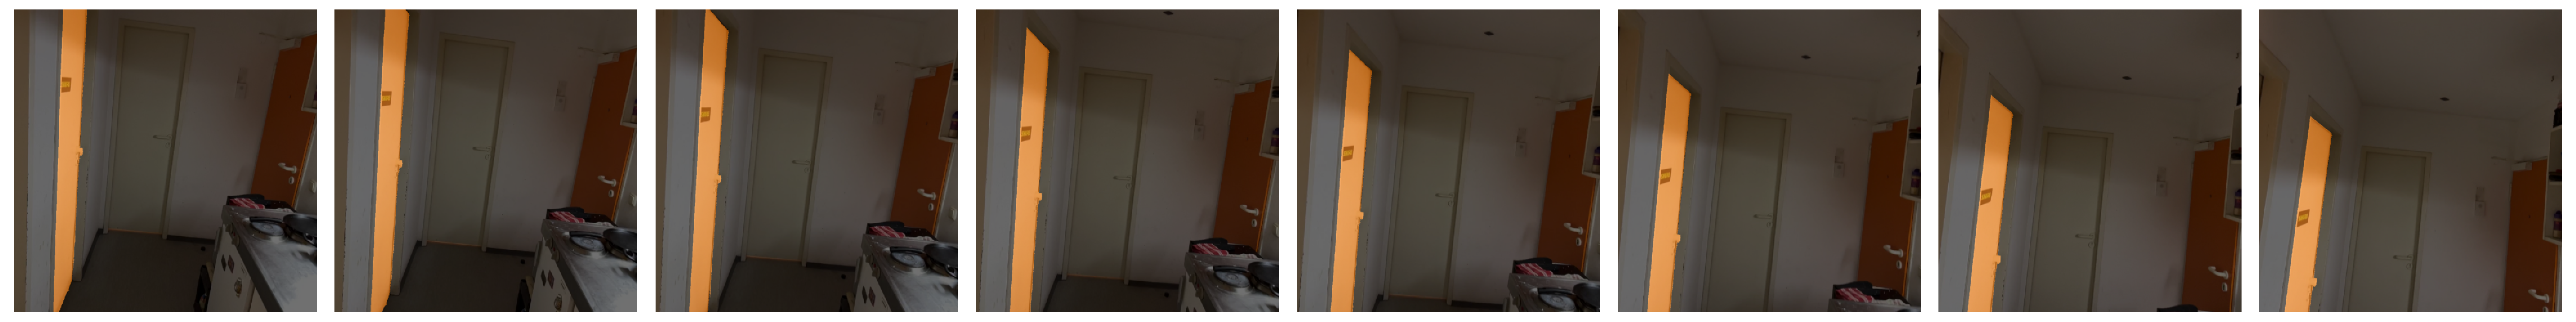
\includegraphics[width=\linewidth]{figs/scanpp_sample_continuous_sampling.pdf}
    \caption{\centering Vanilla continuous sampling strategy}
    \label{fig:cont-samp}
  \end{subfigure}
  \begin{subfigure}{\linewidth}
    \captionsetup{justification=raggedright,singlelinecheck=false}
    % \vspace{-12pt} % tighten space between caption and image
    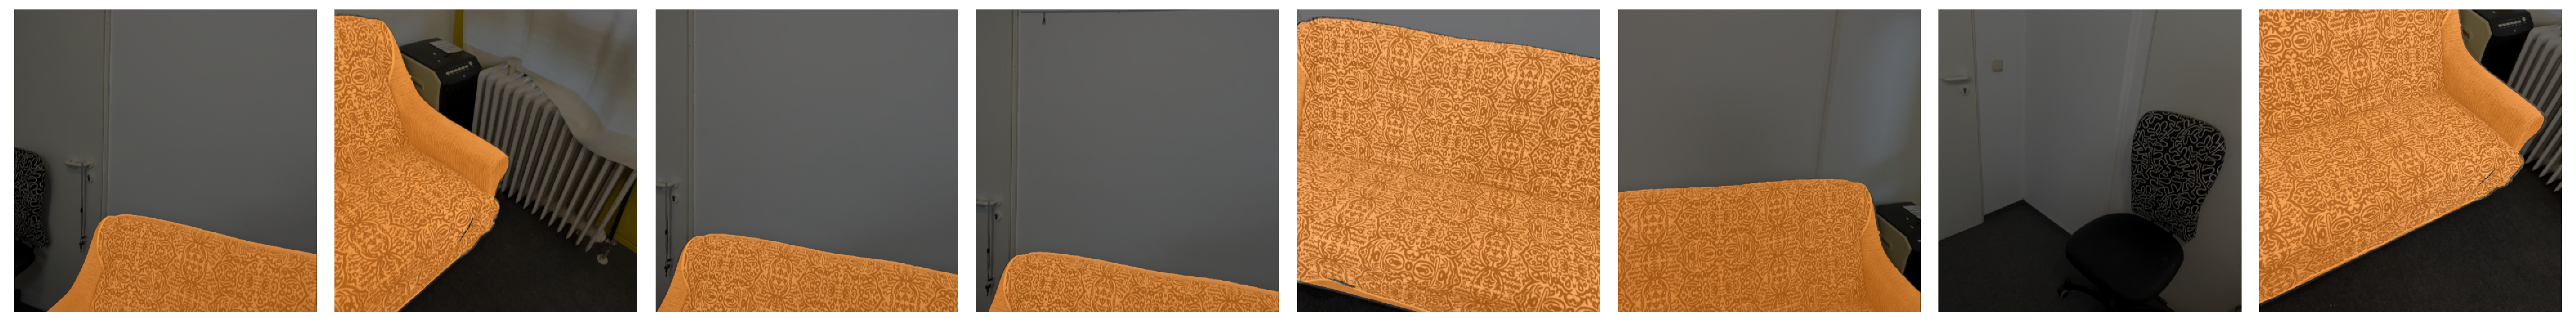
\includegraphics[width=\linewidth]{figs/scanpp_sample_no_fov_sampling.pdf}
    \caption{\centering Naive random sampling without considering field-of-view}
    \label{fig:rand-samp}
  \end{subfigure}
  \begin{subfigure}{\linewidth}
    \captionsetup{justification=raggedright,singlelinecheck=false}
    % \vspace{-12pt}
    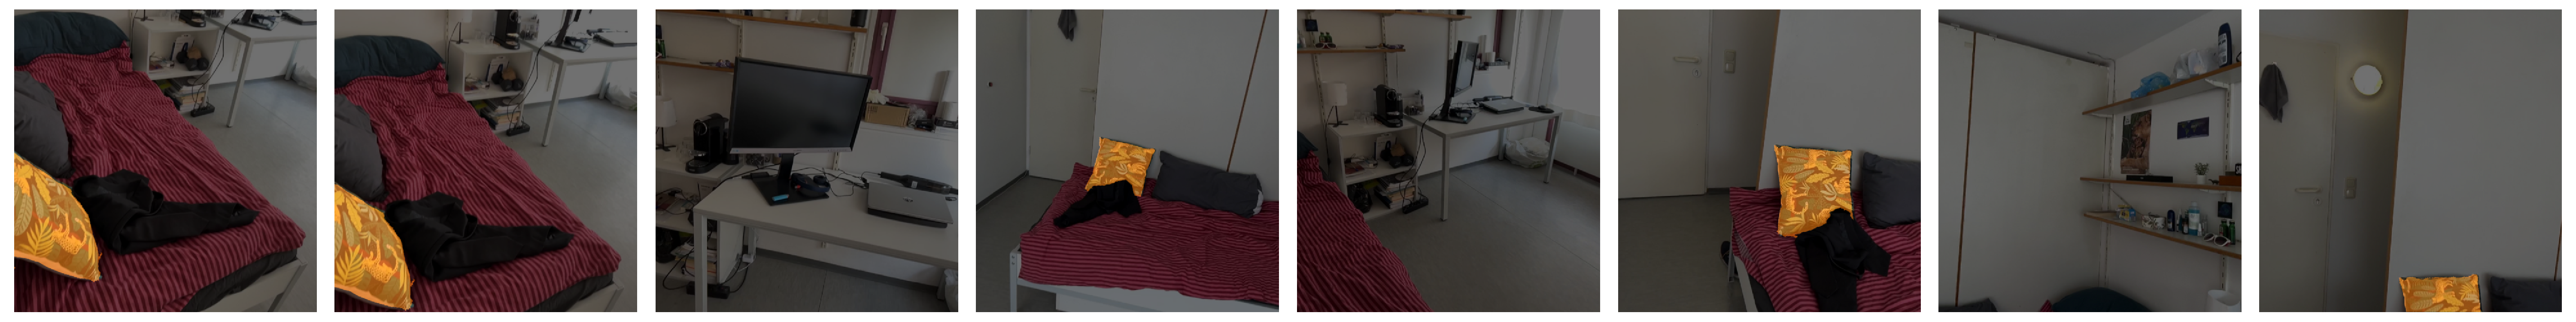
\includegraphics[width=\linewidth]{figs/scanpp_sample_fov_sampling.pdf}
    \caption{\centering Field-of-view–aware sampling strategy (Ours)}
    \label{fig:fov-samp}
  \end{subfigure}
\vspace{-6mm}
    \caption{\textbf{Overview of our sampling strategy during training.}
    (a) Continuous sampling provides densely spaced frames but offers limited viewpoint diversity.
    (b) Naïve random sampling introduces viewpoint variation but may select frames that observe spatially disjoint regions of the same object.  
    For example, frame~0 shows the left side of the couch while frame~1 shows the right side.  
    Because these regions are far apart in 3D space, treating them as the same supervisory signal forces the model to match inconsistent geometry and leads to ambiguous learning.
    (c) Our field-of-view–aware sampling retains only frames whose masked 3D points lie within the reference camera frustum over a threshold, ensuring consistent geometric overlap while preserving natural pose and occlusion variation.}

  \label{fig:pipeline}
\vspace{-3mm}
\end{figure*}


A key challenge in training our model is the limited capacity of the memory module 
(SAM2 maintains at most eight memory slots).  
To enable the model to learn robust object identification across diverse camera viewpoints, 
we must carefully design how training frames are sampled from each video sequence.

\vspace{-1em}
\subsubsection{Naïve Random Sampling.}
A straightforward strategy is to randomly sample $N$ frames from the video as in \cref{fig:rand-samp}.
This exposes the model to a broad distribution of camera viewpoints and object appearances.  
Random sampling also naturally introduces distracting or visually similar objects in the scene 
, which encourages the model to rely on 3D-aware alignment rather than purely local 2D similarity.

\vspace{-1em}
\subsubsection{Object Spanning Problem.}
However, naïve random sampling introduces a failure mode when an object occupies a large spatial extent.  
Consider a bed, table, or cabinet: two randomly sampled frames may both contain the same instance, 
yet correspond to spatially distant regions (e.g., one frame at the headboard, the other at the footboard). 
Since our objective is to enforce 3D location consistency, which is to encourage the model to identify an object by recognizing that it lies in the nearby 3D position; thus, these wide-baseline views of a large object may contradict the intended training signal.  
Although the two frames belong to the same instance, their projected 3D locations are far apart, which can confuse the learning objective.

\vspace{-1em}
\subsubsection{Field-of-View Sampling.}
For each training iteration, the first sampled frame is designated as the reference frame.  
To select the remaining $N\!-\!1$ frames, we apply a FOV-based filter using camera poses and depth.  
For every candidate frame, we back-project its object mask into 3D, transform the points into the reference frame, and re-project them onto the reference image.  
A frame is kept only if a sufficient fraction of its masked 3D points fall inside the reference camera frustum:
\[
\frac{\#\{\text{candidate masked points inside reference frustum}\}}
       {\#\{\text{masked points in candidate frame}\}}
> \tau.
\]
This ensures that selected frames observe overlapping physical regions of the object, avoiding degenerate cases where two views of the same instance correspond to distant, non-overlapping parts.  
We do not filter out partially occluded frames: frustum overlap reflects alignment in viewing direction, not full visibility, and retaining occlusion cases helps the model learn to differentiate viewpoint changes from true object absence.

Note that we apply FoV Sampling as a filter only when candidate masks contain an object. For no-object frames, which are also sampled during training, the model is simply required to predict target absence. In these cases, spatial distance does not affect the objective. That is, when views are far apart, the prediction is driven by geometric inconsistency, while for nearby views, it relies on appearance cues.

We describe our final sampling policy and its ablations in \cref{sec:exp}.

\vspace{-0.5em}
\subsection{Dynamic Object Fallback}
\vspace{-0.5em}
An intuitive limitation of our method lies in dynamic objects, whose shape, location, or orientation may change over time. Such scenarios are prevalent in traditional VOS benchmarks~\cite{perazzi2017davis, xu2018youtube, fan2019lasot}. 
Our approach relies heavily on relative appearance with respect to surrounding geometry (i.e., consistent geometrical locations across views). 
When an object undergoes significant motion, this assumption may break, potentially leading to tracking failure.
To address this issue, we detect the presence of motion using~\cite{Huang_2025_seganymotion} and revert to the original SAM2 pipeline when substantial motion is observed. 
Since the SAM2 image encoder remains frozen in our framework, we can reuse the visual feature and the additional computational overhead incurred by memory attention and mask decoder is negligible.

Empirically, we observed that dynamically toggling between 3AM and vanilla SAM2 mid-sequence (\eg, with a simple motion detection branch before mask decoder) corrupts the temporal memory bank, as the two pathways produce fundamentally different mask distributions. Therefore, we utilize a simple sequence-level fallback to the original SAM2 pipeline when substantial motion is detected. 
This design choice is grounded in a practical categorization of tracking scenarios based on the object's 
visibility with respect to the camera frustum: 
(1) \textit{Dynamic object with continuous visibility}, where the object remains within the camera frustum and 
vanilla SAM2 performs well; 
(2) \textit{Static object with temporary disappearance}, where the object leaves the camera frustum and later 
re-enters, resulting in a re-identification problem that 3AM is designed to address; and 
(3) \textit{Dynamic object with unobserved motion outside the frustum}. 

The third scenario represents an inherently ill-posed problem, as the object may move unpredictably while 
unobserved outside the camera frustum. Consequently, reliable tracking is fundamentally impossible. Since this 
extreme scenario cannot be effectively solved, engineering a complex mid-sequence fusion module is unnecessary. 
Hence a simple sequence-level switch is sufficient to cover the two tractable scenarios.